% !Mode:: "TeX::UTF-8"

\documentclass{svk_short_sk}
%% ak pisete po anglicky, pouzijete namiesto horneho riadku
%% \documentclass{svk_short_en}

\begin{document}
\title{Zarovnávanie sekvencií s použitím metód klasifikácie}

\author{Michal Hozza
\email{Michal.Hozza@ksp.sk}
}
%% vsimnite si, ze u autorov sa nepisu tituly
%% prikaz \inst sluzi ako odkaz do zoznamu institucii
%% (vid. nizsie)

%% skolitela nepiste medzi autorov, ale v tejto casti
%% ak praca nema skolitela, jednoducho vynechajte
\supervisor{Tomáš Vinař\inst{1}
\email{vinar@fmph.uniba.sk}
, Michal N\'an\'asi\inst{2}
\email{mic@compbio.fmph.uniba.sk}
}

%% nasleduje kratka verzia nazvu clanku a
%% zoznam autorov (bez krstnych mien)
%% tieto informacie sa zobrazuju v hlavicke
\titlerunning{Zarovnávanie sekvencií s použitím metód klasifikácie}
\authorrunning{Hozza}

\institute{
Katedra aplikovanej informatiky,
FMFI UK,
Mlynská Dolina
842~48~Bratislava
\and
Katedra informatiky,
FMFI UK,
Mlynská Dolina
842~48~Bratislava}

\maketitle

Bežné zarovnávače DNA sekvencií pracujú len s jednotlivými dvojicami báz \cite{durbin}. Naše zakomponováva dodatočné informácie (poskytnuté formou anotácií k bázam), aby sme vytvorili kvalitnejšie zarovnania.


Na zakomponovanie informácie sme sa rozhodli využiť klasifikátory, ktoré rozhodujú, či dané pozície majú byť zarovnané k sebe alebo nie.

Vyvinuli sme 2 modely pre zarovnanie sekvencií s anotáciami za pomoci klasifikátora, ktoré sú založené na skrytých Markvovych modeloch.

\textbf{Model s klasifikátorom ako emisiou:}
V tomto modeli sme nahradili emisné tabuľky stavov výstupom z klasifikátora.

\begin{figure}[htp]
    \centering
    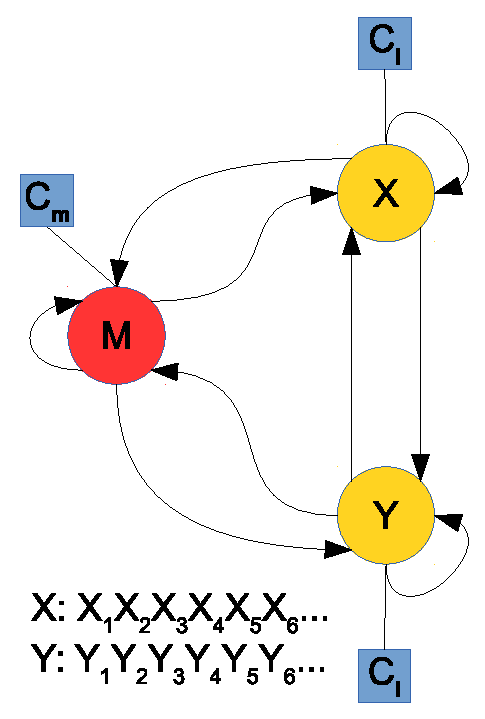
\includegraphics[width=.3\textwidth]{images/model_clf}
    \caption{Model s klasifikátorom ako emisiou}
\end{figure}

Problémom tohto modelu je, Model však nie je celkom korektný, pretože pravdepodobnosti emisií nesumujú do 1. Avšak ukázalo sa, že model aj napriek tomu funguje celkom dobre.

V tomto modeli sme trénovali iba tranzície, emisie sme mali priamo z natrénovaného klasifikátora.

\textbf{Model s klasifikátorovou páskou:}
Aby sme vyriešili problém s korektnosťou predošlého modelu, navrhli sme alternatívny model, ktorý navyše modeluje aj výstup z klasifikátora.
Nemodelujeme teda len dvojicu sekvencií, ale aj sekvenciu výstupov klasifikátora.

\begin{figure}[htp]
    \centering
    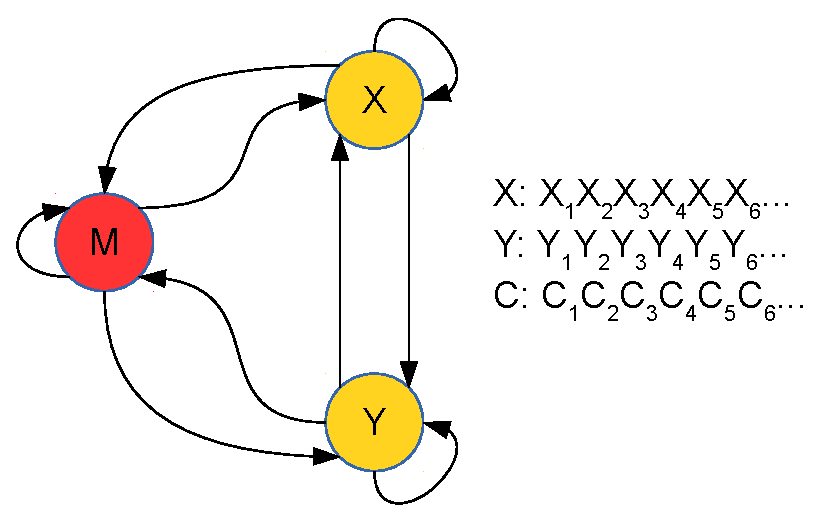
\includegraphics[width=.3\textwidth]{images/model_clf_paska}
    \caption{Model s klasifikátorovou páskou}
\end{figure}

V tomto modeli sme trénovali aj tranzície aj emisie. Výstupy z klasifikátora sme rozdelili do 10 košov rovnomerne na intervale <0, 1>

\begin{figure}[htp]
    \centering
    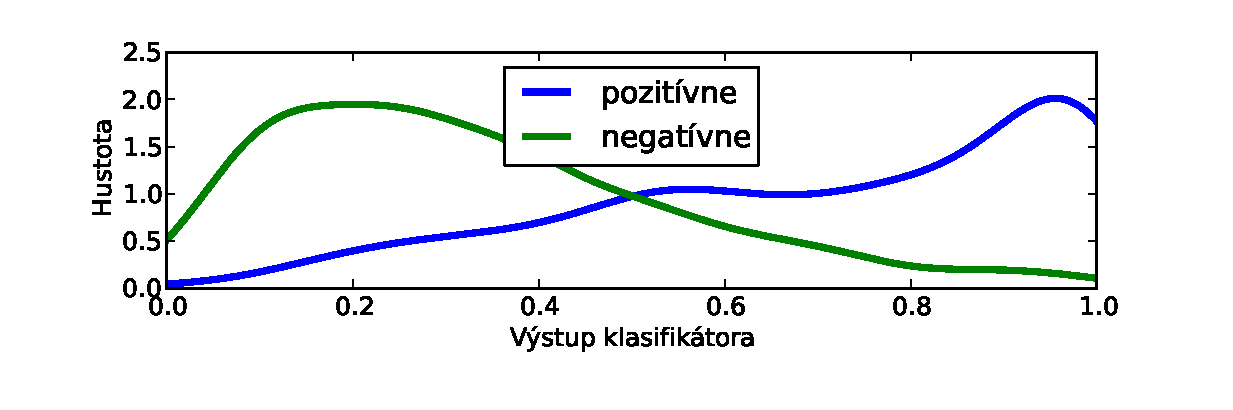
\includegraphics[width=.3\textwidth]{images/clf_m_test}
    \caption{Distribúcia výstupu klasifikátora pre pozitívne (modrá) a negatívne (zelená) príklady}
    \label{fig:clf-m-dist}
\end{figure}

Ukázalo sa, že klasifikátor sa dokáže celkom dobre naučiť, ktoré bázy majú byť zarovnané k sebe a ktoré nie. Na obrázku \ref{fig:clf-m-dist} je distribúcia výstupov klasifikátora. Pozitívne príklady sú tie, ktoré majú byť zarovnané k sebe.

\nocite{*}
\bibliographystyle{apalike}
\bibliography{references}

%% citacie ulozte do suboru references.bib
%% na populaciu zoznamu literatury pouzite program
%%
%% bibtex references
%%
%% po ktorom je potrebne dokument znova zlatexovat

\end{document}
